\documentclass{beamer}
\usepackage{tikz}
\usetikzlibrary{calc}
\usepackage{xcolor}
\usepackage{multicol}
\usepackage{amsmath}

\title{Fractions: Of Amounts \& Multiplying}
\author{}
\date{}

\begin{document}

\frame{\titlepage}

%------------------------------------------------
% SLIDE 15: Fractions of Amounts (Introduction)
%------------------------------------------------
\begin{frame}{Starter}

\vspace{-2em}

\begin{columns}

\column{0.25\textwidth}
\begin{center}
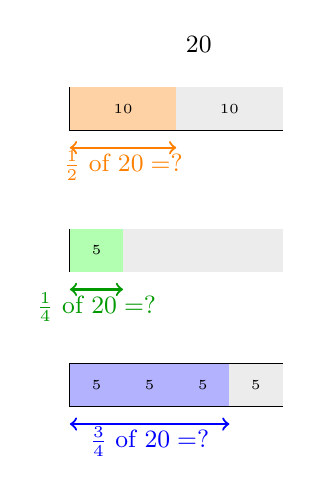
\begin{tikzpicture}[scale=0.9]

% Label for whole (20) above the top bar
\node[anchor=west] at (1.5,5.0) {\small $20$};

% Bar model for 1/2 of 20 (top)
\draw (0,3.8) rectangle (3,4.4);
\draw (1.5,3.8) -- (1.5,4.4);
\fill[orange!35] (0,3.8) rectangle (1.5,4.4);
\fill[gray!15] (1.5,3.8) rectangle (3,4.4);
\node at (0.75,4.1) {\tiny $10$};
\node at (2.25,4.1) {\tiny $10$};

\draw[<->, orange, thick] (0,3.55) -- (1.5,3.55);
\node[orange] at (0.75,3.3) {\small $\frac{1}{2}$ of $20 = ?$};

% Bar model for 1/4 of 20 (middle)
\draw (0,1.8) rectangle (3,2.4);
\foreach \x in {0.75,1.5,2.25} \draw (\x,1.8) -- (\x,2.4);
\fill[green!30] (0,1.8) rectangle (0.75,2.4);
\fill[gray!15] (0.75,1.8) rectangle (3,2.4);
\node at (0.375,2.1) {\tiny $5$};

\draw[<->, green!60!black, thick] (0,1.55) -- (0.75,1.55);
\node[green!60!black] at (0.375,1.3) {\small $\frac{1}{4}$ of $20 = ?$};

% Bar model for 3/4 of 20 (bottom)
\draw (0,-0.1) rectangle (3,0.5);
\foreach \x in {0.75,1.5,2.25} \draw (\x,-0.1) -- (\x,0.5);
\fill[blue!30] (0,-0.1) rectangle (2.25,0.5);
\fill[gray!15] (2.25,-0.1) rectangle (3,0.5);
\node at (0.375,0.2) {\tiny $5$};
\node at (1.125,0.2) {\tiny $5$};
\node at (1.875,0.2) {\tiny $5$};
\node at (2.625,0.2) {\tiny $5$};

\draw[<->, blue, thick] (0,-0.35) -- (2.25,-0.35);
\node[blue] at (1.125,-0.6) {\small $\frac{3}{4}$ of $20 = ?$};

\end{tikzpicture}
\end{center}

\column{0.75\textwidth}
\small
\begin{enumerate}
\begin{multicols}{2}
  \item Fully simplify: $\dfrac{18}{24}$
  \item Calculate: $2\dfrac{1}{3} + 1\dfrac{1}{2}$
\end{multicols}
  \item Using the bar models to the left:
  \[
    \tfrac{1}{2} \text{ of } 20 = \square \qquad \tfrac{1}{4} \text{ of } 20 = \square \qquad \tfrac{3}{4} \text{ of } 20 = \square
  \]
  \item Calculate:
  \[
    \tfrac{1}{3} \text{ of } 24 \qquad \tfrac{2}{3} \text{ of } 24
  \]
  \item Fill in the blank: $\quad \dfrac{3}{4}$ of $\square = 18$
  \item True or false? ``$\dfrac{1}{2}$ of $30 = 30 \div 2$.'' Explain your reasoning.
\begin{multicols}{2}
  \item Find $\dfrac{2}{5}$ of $35$.
  \vspace{2em}
  \item A $60\,\text{cm}$ ribbon is cut. Amy takes $\dfrac{3}{4}$ of it. How long is her piece?
\end{multicols}
\end{enumerate}
\end{columns}
\end{frame}


%------------------------------------------------
% SLIDE 16: Fractions of Amounts (Mixed difficulty)
%------------------------------------------------
\begin{frame}{Starter}

\vspace{-2em}

\begin{columns}

\column{0.22\textwidth}
\begin{center}
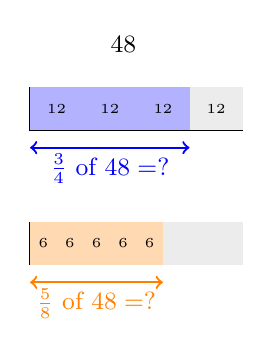
\begin{tikzpicture}[scale=0.9]

% Bar model for 3/4 of 48
\node[anchor=west] at (1, 5.5) {\small $48$};

\draw (0,4.3) rectangle (3,4.9);
\foreach \x in {0.75,1.5,2.25} \draw (\x,4.3) -- (\x,4.9);
\fill[blue!30] (0,4.3) rectangle (0.75,4.9);
\fill[blue!30] (0.75,4.3) rectangle (1.5,4.9);
\fill[blue!30] (1.5,4.3) rectangle (2.25,4.9);
\fill[gray!15] (2.25,4.3) rectangle (3,4.9);
\node at (0.375,4.6) {\tiny $12$};
\node at (1.125,4.6) {\tiny $12$};
\node at (1.875,4.6) {\tiny $12$};
\node at (2.625,4.6) {\tiny $12$};

\draw[<->, blue, thick] (0,4.05) -- (2.25,4.05);
\node[blue] at (1.125,3.75) {\small $\frac{3}{4}$ of $48 = ?$};


\draw (0,2.4) rectangle (3,3.0);
\foreach \x in {0.375,0.75,1.125,1.5,1.875,2.25,2.625} \draw (\x,2.4) -- (\x,3.0);
\fill[orange!30] (0,2.4) rectangle (1.875,3.0);
\fill[gray!15] (1.875,2.4) rectangle (3,3.0);
\node at (0.1875,2.7) {\tiny $6$};
\node at (0.5625,2.7) {\tiny $6$};
\node at (0.9375,2.7) {\tiny $6$};
\node at (1.3125,2.7) {\tiny $6$};
\node at (1.6875,2.7) {\tiny $6$};

\draw[<->, orange, thick] (0,2.15) -- (1.875,2.15);
\node[orange] at (0.9375,1.85) {\small $\frac{5}{8}$ of $48 = ?$};


\end{tikzpicture}
\end{center}

\column{0.78\textwidth}
\small
\begin{enumerate}
  \item Order smallest to largest: $\dfrac{3}{8},\ \dfrac{1}{2},\ \dfrac{5}{12}$
  \item Convert $\dfrac{17}{5}$ to a mixed number.
  \item Use the bar model to find $\dfrac{3}{4}$ of $48$ and $\dfrac{5}{8}$ of $48$.
  \item Calculate: $\quad \dfrac{5}{8}$ of $72$
  \item $\dfrac{2}{3}$ of a class of $30$ are girls. How many boys are there?
  \item Rania says ``$\dfrac{3}{5}$ of $40 = 24$''. Is she correct? Show your working.

\begin{multicols}{2}
  \item Which is greater: \newline $\dfrac{3}{4}$ of $60$ or $\dfrac{4}{5}$ of $55$?
  \item Fill in the blank:
  \[
    \frac{\square}{8} \text{ of } 64 = 40
  \]
\end{multicols}
\end{enumerate}
\end{columns}
\end{frame}


%------------------------------------------------
% SLIDE 17: Multiplying Fractions (Introduction)
%------------------------------------------------
\begin{frame}{Starter}

\vspace{-2em}

\begin{columns}

\column{0.25\textwidth}
\begin{center}
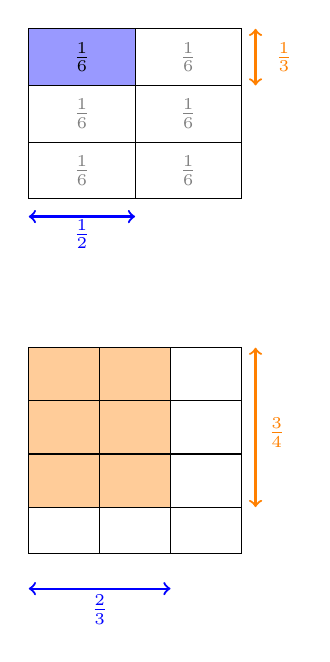
\begin{tikzpicture}[scale=0.9]

% Area model for 1/2 x 1/3


% Grid: 2 columns x 3 rows = 6 cells
\draw (0,2.5) rectangle (3,4.9);
% vertical line (halves)
\draw (1.5,2.5) -- (1.5,4.9);
% horizontal lines (thirds)
\draw (0,3.3) -- (3,3.3);
\draw (0,4.1) -- (3,4.1);

% shade 1 cell (top-left = 1/2 wide, 1/3 tall)
\fill[blue!40] (0,4.1) rectangle (1.5,4.9);

\node at (0.75,4.5) {\small $\frac{1}{6}$};
\node[gray] at (2.25,4.5) {\small $\frac{1}{6}$};
\node[gray] at (0.75,3.7) {\small $\frac{1}{6}$};
\node[gray] at (2.25,3.7) {\small $\frac{1}{6}$};
\node[gray] at (0.75,2.9) {\small $\frac{1}{6}$};
\node[gray] at (2.25,2.9) {\small $\frac{1}{6}$};

% labels on axes
\draw[<->, blue, thick] (0,2.25) -- (1.5,2.25);
\node[blue] at (0.75,2.0) {\small $\frac{1}{2}$};
\draw[<->, orange, thick] (3.2,4.1) -- (3.2,4.9);
\node[orange] at (3.6,4.5) {\small $\frac{1}{3}$};


% Area model for 2/3 x 3/4

\draw (0,-2.5) rectangle (3,0.4);
% shade 2/3 wide x 3/4 tall = 6 of 12 cells
\fill[orange!40] (0,-1.85) rectangle (2,0.4);

% vertical lines (thirds)
\draw (1,  -2.5) -- (1,  0.4);
\draw (2,  -2.5) -- (2,  0.4);
% horizontal lines (quarters)
\draw (0,-0.35) -- (3,-0.35);
\draw (0,-1.1) -- (3,-1.1);
\draw (0,-1.85) -- (3,-1.85);

% labels on axes
\draw[<->, blue, thick] (0,-3.0) -- (2,-3.0);
\node[blue] at (1,-3.3) {\small $\frac{2}{3}$};
\draw[<->, orange, thick] (3.2,0.4) -- (3.2,-1.85);
\node[orange] at (3.5,-0.8) {\small $\frac{3}{4}$};



\end{tikzpicture}
\end{center}

\column{0.75\textwidth}
\small
\begin{enumerate}
  \item What is $\dfrac{1}{2}$ of $\dfrac{1}{2}$? Draw a picture to show your answer.
  \item Use the area model on the left to calculate $\dfrac{1}{2} \times \dfrac{1}{3} = \dfrac{\square}{\square}$
  \item Use the second area model to calculate and simplify: $\dfrac{2}{3} \times \dfrac{3}{4} = \dfrac{\square}{\square} = \dfrac{\square}{\square}$
  \item Calculate:
  \[
    \frac{3}{5} \times \frac{5}{7}
  \]
  \item Simplify \textit{then} multiply: $\quad\dfrac{3}{9} \times \dfrac{4}{8}$
  \item Find $\dfrac{3}{4}$ of $\dfrac{2}{5}$. What do you notice about ``of'' and ``$\times$''?
  \item Calculate: $1\dfrac{1}{2} \times \dfrac{1}{3}$\\[0.3em]
  (Hint: convert to improper first.)
\end{enumerate}
\end{columns}
\end{frame}


%------------------------------------------------
% SLIDE 18: Multiplying Fractions & Amounts (Mixed)
%------------------------------------------------
\begin{frame}{Starter}

\vspace{-2em}

\begin{columns}

\column{0.22\textwidth}
\begin{center}
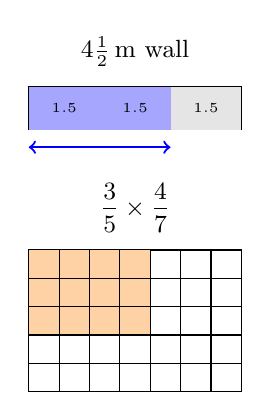
\begin{tikzpicture}[scale=0.9]

% Illustration: 2/3 of 4.5m wall
\node at (1.5, 5.3) {\small $4\tfrac{1}{2}$\,m wall};

\draw (0,4.2) rectangle (3,4.8);
\foreach \x in {1,2} \draw (\x,4.2) -- (\x,4.8);
\fill[gray!20] (0,4.2) rectangle (3,4.8);
\fill[blue!35] (0,4.2) rectangle (2,4.8);
\node at (0.5,4.5) {\tiny $1.5$};
\node at (1.5,4.5) {\tiny $1.5$};
\node at (2.5,4.5) {\tiny $1.5$};

\draw[<->, blue, thick] (0,3.95) -- (2,3.95);


% Area model reminder: 3/5 x 4/7
\node at (1.5,3.1) {\small $\dfrac{3}{5} \times \dfrac{4}{7}$};

\draw (0,0.5) rectangle (3,2.5);
\fill[orange!35] (0,1.3) rectangle (1.7143,2.5);

% 5 rows, 7 cols
\foreach \y in {0.9,1.3,1.7,2.1} \draw (0,\y) -- (3,\y);
\foreach \x in {0.4286,0.8571,1.2857,1.7143,2.1429,2.5714} \draw (\x,0.5) -- (\x,2.5);



\end{tikzpicture}
\end{center}

\column{0.78\textwidth}
\small
\begin{enumerate}
\begin{multicols}{3}
  \item Simplify: $\dfrac{24}{36}$
  \item $3\dfrac{1}{4} - 1\dfrac{2}{3}$
  \item $\dfrac{5}{6}$ of $42$
\end{multicols}


  \item A wall is $4\dfrac{1}{2}$\,m long. A mural covers $\dfrac{2}{3}$ of it. Use the bar model to find the length of the mural.


  \item Use the area model to calculate: $\dfrac{3}{5} \times \dfrac{4}{7} = \dfrac{\square}{\square}$

  \item Which is greater: $\dfrac{2}{3} \times \dfrac{3}{4}$, or $\dfrac{3}{4}$ of $\dfrac{2}{3}$? Explain.

\begin{multicols}{2}
  \item Fill in the blank:
  \[
    \frac{3}{5} \times \square = \frac{6}{35}
  \]
  \newline
  \item True or false? ``Multiplying two proper fractions always gives a smaller result than either fraction.'' Explain or give a counterexample.
\end{multicols}
\end{enumerate}
\end{columns}
\end{frame}


%------------------------------------------------
% SLIDE 19: Problem Solving & Mastery
%------------------------------------------------
\begin{frame}{Starter}

\vspace{-2em}

\begin{columns}

\column{0.22\textwidth}
\begin{center}
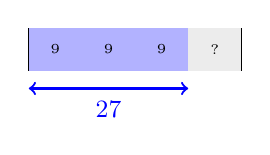
\begin{tikzpicture}[scale=0.9]

% Bar model: 3/4 of a number is 27

\draw (0,3.7) rectangle (3,4.3);
\foreach \x in {0.75,1.5,2.25} \draw (\x,3.7) -- (\x,4.3);
\fill[blue!30] (0,3.7) rectangle (2.25,4.3);
\fill[gray!15] (2.25,3.7) rectangle (3,4.3);
\node at (0.375,4.0) {\tiny $9$};
\node at (1.125,4.0) {\tiny $9$};
\node at (1.875,4.0) {\tiny $9$};
\node at (2.625,4.0) {\tiny $?$};

\draw[<->, blue, thick] (0,3.45) -- (2.25,3.45);
\node[blue] at (1.125,3.15) {\small $27$};


\end{tikzpicture}
\end{center}

\column{0.78\textwidth}
\small
\begin{enumerate}
\begin{multicols}{3}
  \item Simplify: $\dfrac{20}{30}$
  \item Simplify: $\dfrac{84}{108}$
\end{multicols}

  \item Convert $4\dfrac{3}{5}$ to an improper fraction.


  \item Calculate: $2\dfrac{3}{4} + 1\dfrac{3}{5}$

  \item $\dfrac{3}{4}$ of a number is $27$. Use the bar model to find the whole number.

  \item Jack spends $\dfrac{1}{3}$ of his pocket money on Monday and $\dfrac{1}{4}$ on Tuesday. What fraction remains?

  \item A jug holds $1\dfrac{1}{2}$ litres. You fill $\dfrac{2}{3}$ of it. How many millilitres is that?

  \item Show that $\dfrac{2}{3} \times \dfrac{3}{4} = \dfrac{3}{4} \times \dfrac{2}{3}$ using area diagrams.


\end{enumerate}
\end{columns}
\end{frame}

\end{document}